\subsection{Bahasa Deskripsi Hardware: Verilog}

Selain menggunakan skematik, desain rangkaian digital juga dapat dilakukan
dengan menggunakan HDL (\textit{hardware description language})
seperti Verilog dan VHDL.
Pada kesempatan kali ini kita akan menggunakan Verilog.

Verilog pada awalnya dikembangkan sebagai alat untuk simulasi serta
verifikasi dari rangkaian digital.
Verilog dikembangkan oleh Gateway Design Automation, yang
sekarang menjadi bagian dari Cadence Design Systems.
Pada awal perkembangannya Verilog merupakan bahasa
proprietary, akan tetapi pada
tahun 1990 Verilog dilepaskan ke
domain publik. Sejak saat itu Verilog menjadi salah satu
bahasa yang populer untuk mendeskripsikan rangkaian digital.
Pada tahun 1995 Verilog diadopsi sebagai IEEE Standard, yaitu standard
1364-1995. Pada tahun 2001, versi terbaru dari Verilog yang dikenal dengan
Verilog 2001 diadopsi menjadi IEEE Standard 1364-2001.

Pada Quartus Prime, file Verilog dapat ditambahkan ke Project
dengan memilih menu \textbf{File $\rightarrow$ New} dan pilih
\textbf{Verilog HDL File}.

\begin{figure}[H]
\centering
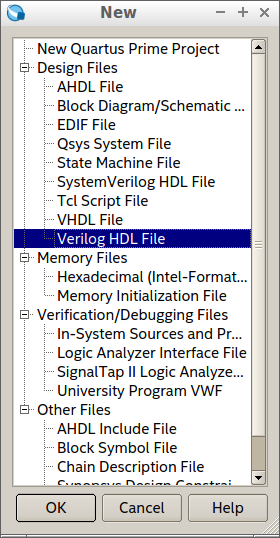
\includegraphics[scale=0.5]{images/new_file_verilog.png}
\par
\caption{New File Verilog HDL}
\end{figure}

File Verilog merupakan file teks sehingga kita dapat menggunakan
teks editor apa saja untuk mengedit file ini.

\subsubsection{Representasi rangkaian digital dengan Verilog}

Terdapat dua pendekatan yang akan kita gunakan untuk mendesain rangkaian
digital dengan Verilog pada praktikum ini
\begin{itemize}

\item struktural: rangkaian digital dideskripsikan dengan struktur
rangkaian tersebut, membangunnya
dengan elemen-elemen rangkaian seperti gerbang logika, dan mendefisinikan
bagaimana elemen-elemen tersebut saling terhubung satu sama lainnya.

\item perilaku (behavioral): rangkaian digital dideskripsikan dengan
perilaku rangkaian tersebut, bukan dengan struktur rangkaiannya secara
langsung. Pendekatan ini dilakukan dengan menggunakan konstruksi
pemrograman Verilog seperti konstruksi \textbf{if}, \textbf{switch}, dan
\textbf{for} yang juga biasa ditemukan pada bahasa
pemrograman komputer. Kompiler Verilog akan melakukan translasi
dari konstruksi pemrograman tersebut menjadi rangkaian digital yang sesuai.z

\end{itemize}


\textbf{Representasi struktural}

Verilog memiliki gerbang logika primitif yang merepresentasikan
gerbang logika yang biasa dipakai pada rangkaian.

Gerbang AND dengan dua input, $x_1$ dan $x_2$,
dan output $y$, misalnya dapat dinyatakan dengan kode Verilog
sebagai berikut.
\begin{verilogcode}
and( y, x1, x2 );
\end{verilogcode}

Gerbang OR dengan 4 input
\begin{verilogcode}
or( y, x1, x2, x3 x4 );
\end{verilogcode}

Inverter $y = \bar{x}$
\begin{verilogcode}
not( y, x );
\end{verilogcode}

Beberapa gerbang primitif pada Verilog dapat diberikan
pada tabel berikut ini.
\begin{table}[h!]
\centering
\begin{tabular}{|ccc|}
\hline
Nama & Deskripsi & Penggunaan \\
\hline\hline
and & $f = (a \cdot b \cdots )$ & \verb|and(f, a, b, ...)| \\
nand & $f = \overline{(a \cdot b \cdots)}$ & \verb|nand(f,a,b,...)| \\
or & $f = (a + b + \cdots)$ & \verb|or(a,b,...)| \\
nor & $f = \overline{(a + b + \cdots)}$ & \verb|nor(a,b,...)| \\
xor & $f = a \oplus b \oplus \cdots $ & \verb|xor(a,b,...)| \\
xnor & $f = a \odot b \odot \cdots $ & \verb|xnor(a,b,...)| \\
not & $f = \bar{a}$ & \verb|not(f,a)| \\
\hline
\end{tabular}
\par
\caption{Beberapa gerbang primitif pada Verilog}
\end{table}

Rangkaian digital yang lebih kompleks
dapat direpresentasikan dengan menggunakan gerbang primitif tersebut.

Dalam tulisan ini, penjelasan mengenai Verilog akan diberikan
melalui contoh.

\begin{figure}[h]
\centering
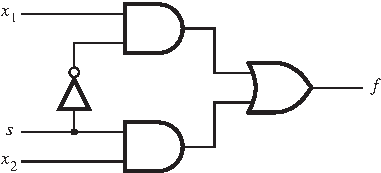
\includegraphics[scale=1.0]{images/fig_2_36.pdf}
\par
\caption{Multiplexer}\label{fig:mux2}
\end{figure}

\framebox[1.1\width]{Contoh 1} Multiplexer pada
Gambar \ref{fig:mux2} dapat dijelaskan dengan kode Verilog berikut.

{\setstretch{1.0}
\begin{verilogcode}
module mux2( x1, x2, s, f );
  input x1, x2, s;
  output f;

  not(k,s);
  and(g,k,x1);
  and(h,s,x2);
  or(f,g,h);
endmodule
\end{verilogcode}
}

Dalam Verilog, rangkaian logika diberikan dalam bentuk modul, didefinisikan
dengan
kata kunci {\tt \textbf{module}}. Suatu modul dapat terdiri dari input dan
output yang disebut sebagai \textit{port}.
Pada contoh di atas, modul dengan nama {\tt \textbf{mux2}} didefinisikan.
Modul {\tt \textbf{mux2}} memiliki 4 port yang bernama {\tt x1}, {\tt x2},
{\tt s}, dan {\tt f}. Pernyataan modul ini diakhiri dengan titik koma.
Pada pernyataan berikutnya, {\tt x1}, {\tt x2} dan {\tt s} dinyatakan
sebagai sinyal input, sedangkan $f$ sebagai sinyal output. Empat baris kode
berikutnya menyatakan struktur dari rangkaian.

Variabel $k$, $g$, dan $h$ tidak dideklarasikan pada kode di atas. Secara default
tipe dari variabel tersebut adalah {\tt wire}.

\framebox[1.1\width]{Contoh 2} Perhatikan rangkaian berikut.

\begin{figure}[H]
\centering
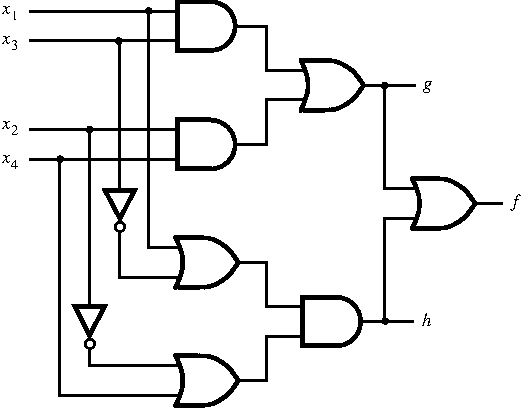
\includegraphics[scale=1.0]{images/fig_2_39.pdf}
\par
\caption{Rangkaian untuk Contoh 2}\label{fig:Contoh2}
\end{figure}

Rangkaian ini memiliki 4 input, yaitu $x_1$, $x_2$, $x_3$, dan
$x_4$, serta 3 output, yaitu $f$, $g$, dan $h$.
Rangkaian ini mengimplementasikan fungsi logika berikut.
\begin{align*}
g & = x_1 x_3 + x_2 x_4 \\
h & = (x_1 + \bar{x_3})(\bar{x_2} + x_4) \\
f & = g + h
\end{align*}

Rangkaian ini dapat diimplementasikan dengan menggunakan kode berikut.
Pada kode ini operator {\tt \textbf{~}} digunakan sebagai pengganti gerbang
NOT.
{\setstretch{1.0}
\begin{verilogcode}
module Contoh2( x1, x2, x3, x4, f, g, h );
  input x1, x2, x3, x4;
  output f, g, h;

  and( z1, x1, x3 );
  and( z2, x2, x4 );
  or( g, z1, z2 );
  or( z3, x1, ~x3 );
  or( z4, ~x2, x4 );
  and( h, z3, z4 );
  or( f, g, h );
endmodule
\end{verilogcode}
}

\textbf{Representasi behavioral}

Menggunakan gerbang logika primitif pada Verilog untuk rangkaian yang
kompleks dapat menjadi tugas yang sulit.
Sebagai alternatif, kita dapat menggunakan ekspresi logika dan
level abtraksi yang lebih tinggi
serta kontruksi pemrograman Verilog untuk mendeskripsikan rangkaian
berdasarkan perilaku dari suatu rangkaian.

Sebagai contoh, output dari multiplexer pada Gambar \ref{fig:mux2}
dapat dijelaskan dengan persamaan logika berikut.
\begin{equation*}
f = \bar{s}x_1 + sx_2
\end{equation*}

Dalam Verilog, persamaan ini dapat dinyatakan dengan kode berikut.
{\setstretch{1.0}
\begin{verilogcode}
module mux2_logic_expr( x1, x3, s, f );
  input x1, x2, s;
  output f;

  assign f = ( ~s & x1 ) | ( s & x2 );
endmodule
\end{verilogcode}
}

Pada kode tersebut, operasi AND dan OR dilakukan dengan menggunakan
operator "{\tt\textbf{\&}}" dan "{\tt\textbf{|}}".

Kata kunci {\tt\textbf{assign}} berarti {\it continuous assignment} untuk
sinyal $f$.
Ketika ada sinyal pada ruas kanan yang berubah, maka $f$ akan dievaluasi ulang.
Jika tidak, maka $f$ akan tetap pada nilai sebelumnya.

Dengan menggunakan ekspresi logika, rangkaian pada Gambar \ref{fig:Contoh2}
dapat dituliskan sebagai berikut.
{\setstretch{1.0}
\begin{verilogcode}
module Contoh2_logic_expr( x1, x2, x3, x4, f, g, h );
  input x1, x2, x3, x4;
  output f, g, h;

  assign g = ( x1 &  x3 ) | (  x2 & x4 );
  assign h = ( x1 | ~x3 ) & ( ~x2 & x4 );
  assign f = g | h;
endmodule
\end{verilogcode}
}

Penggunaan ekspresi logika dapat mempermudah penulisan kode Verilog.
Akan tetapi level abstraksi yang lebih tinggi juga dapat digunakan
dengan cara memberikan spesifikasi mengenai perilaku dari rangkaian.
Rangkaian ini juga dapat dideskripsikan dengan menyatakan perilakunya
sebagai berikut.
\begin{itemize}
\item $f = x_1$ jika $s = 0$, dan
\item $f = x_2$ jika $s = 1$
\end{itemize}

Dalam Verilog, perilaku ini dapat dijelaskan dengan menggunakan
pernyataan {\tt \bf if-else} seperti pada kode berikut.
{\setstretch{1.0}
\begin{verilogcode}
module mux2_behavioral( x1, x2, f );
  input x1;
  input x2;
  output f;

  reg f;

  always @(x1 or x2 or s)
    if( s == 0 )
      f = x1;
    else
      f = x2;
endmodule
\end{verilogcode}
}

Beberapa hal yang perlu diperhatikan terkait kode di atas.

\begin{itemize}
\item Pernyataan {\tt\textbf{if-else}} pada Verilog termasuk dalam
\textit{pernyataan prosedural}.
Verilog mengharuskan pernyataan prosedural diletakkan pada blok
{\tt\textbf{always}},
seperti pada kode di atas. Setiap blok {\tt\textbf{always}} dapat terdiri dari satu
pernyataan, seperti pada contoh di atas, atau beberapa pernyataan prosedural.
Suatu modul Verilog dapat memiliki beberapa
blok {\tt\textbf{always}} yang masing-masing blok tersebut menyatakan suatu bagian
dari rangkaian yang sedang dimodelkan.
\item Pernyataan dalam blok {\tt\textbf{always}} akan dievaluasi sesuai dengan urutan yang
diberikan dalam kode. Hal ini kontras dengan pernyataan
\textit{continuous assignment}
yang dievaluasi secara paralel dan tidak bergantung pada urutan yang diberikan
di kode.
\item Pada blok {\tt\textbf{always}}, setelah simbol {\tt \textbf{@}},
dalam tanda kurung, disebut
dengan \textit{sensitivity list}. Pernyataan pada blok {\tt\textbf{always}} akan dieksekusi
jika satu atau lebih dari sinyal yang ada pada \textit{sensitivity list} berubah.
Hal ini berguna pada waktu simulasi, di mana simulator tidak perlu mengeksekusi
pernyataan setiap waktu.
Untuk keperluan sintesis, \textit{sensitivity list} memberitahu
\textit{compiler} sinyal
apa saja yang secara langsung mempengaruhi keluaran yang diberikan oleh blok
{\tt\textbf{always}}.
\item Jika suatu sinyal diberikan suatu nilai dengan menggunakan pernyataan
prosedural, Verilog mengharuskan sinyal tersebut dideklarasikan sebagai
\textit{variabel}. Hal ini dilakukan dengan cara menggunakan kata kunci
{\tt\textbf{reg}}.
\end{itemize}

\textbf{Mengubah kode Verilog menjadi simbol}

Kode Verilog yang telah dibuat juga dapat digunakan pada skematik yang
lebih besar dengan car mengubah kode Verilog tersebut dengan melalui
menu \textbf{File $\rightarrow$ Create/Update $\rightarrow$ Create Symbol Files
for Current File}.



